\documentclass[tikz,border=10pt]{standalone}
\begin{document}
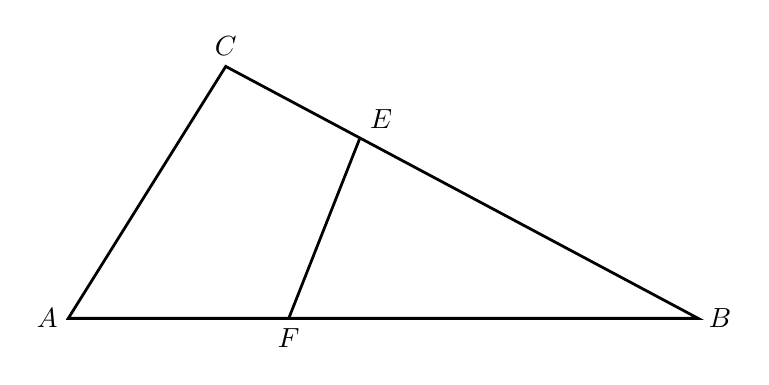
\begin{tikzpicture}[line width=1pt]
\coordinate (A) at (0,0);
\coordinate (B) at (8,0);
\coordinate (C) at (2,3.2);
\coordinate (E) at (3.7,2.28);
\coordinate (F) at (2.8,0);

\draw (A) -- (B) -- (C) -- cycle;
\draw (E) -- (F);

\node[above] at (C) {$C$};
\node[above right] at (E) {$E$};
\node[below] at (F) {$F$};
\node[left] at (A) {$A$};
\node[right] at (B) {$B$};
\end{tikzpicture}
\end{document}
